% colocar las versiones que se realizaran posteriormente hacer referencia en los resultados ponerlo con subsecciones el codigo colocarlo como un apendice colocar un pie de nota de los codigos que se encuentran en mi github no se requiere mencionar librerias en los codigos documentar un poco los codigos
\section{Descripción de los datos}
\label{sec:descripcion-datos}

El análisis exploratorio se desarrolló en \texttt{ventanas.ipynb}, a partir del archivo \texttt{datos.csv}. La salida de lectura conservada en el cuaderno reporta 373\,768 registros y nueve columnas originales. Este conteo corresponde al conjunto completo, antes de seleccionar el área y el periodo de los experimentos.

Cada registro contiene información eléctrica asociada con un sistema, un área y una marca temporal. La inspección inicial muestra registros del 1 de enero de 2020 a las 00:00 y del 30 de septiembre de 2024 a las 23:00. Estos extremos proceden de las filas mostradas por el cuaderno; no sustituyen una comprobación de continuidad temporal para cada área.

\begin{table}[htbp]
\centering
\caption{Variables originales del conjunto de datos.}
\label{tab:variables-originales}
\begin{tabular}{p{0.46\textwidth}p{0.44\textwidth}}
\toprule
Columna & Descripción \\
\midrule
Sistema & Identificador del sistema eléctrico. \\
Area & Identificador del área. \\
Generacion (MWh) & Generación eléctrica; variable de respuesta del OLS actual. \\
Importacion Total (MWh) & Energía importada. \\
Exportacion Total (MWh) & Energía exportada. \\
Intercambio neto entre Gerencias (MWh) & Intercambio neto registrado entre gerencias. \\
Estimacion de Demanda por Balance (MWh) & Estimación de la demanda mediante balance. \\
Pronostico (MWh) & Pronóstico incluido en la fuente de datos. \\
Timestamp & Fecha y hora del registro. \\
\bottomrule
\end{tabular}
\end{table}

Las salidas del agrupamiento identifican nueve áreas: BCA, BCS, CEN, NES, NOR, NTE, OCC, ORI y PEN. Se generó una gráfica de generación para cada una. La primera fila del archivo pertenece a BCA; por ello, la selección del primer valor de \texttt{Area} empleada en los programas corresponde a BCA para el archivo mostrado en el cuaderno.

La marca temporal se interpreta con el formato día/mes/año y hora:minuto. Los registros iniciales exhiben incrementos de una hora. Sin embargo, el número total de filas reúne diferentes áreas y no representa la longitud de una sola serie temporal. Los conteos por área, los valores faltantes y la continuidad de cada serie requieren verificaciones específicas antes del entrenamiento.

\subsection{Agrupamiento y exploración temporal}

Se construyó una tabla agrupada por fecha, hora y área, sumando la generación en cada combinación. La salida conserva 373\,768 filas y tres columnas: fecha y hora, área y generación. El conteo coincide con el de la lectura inicial en la ejecución almacenada.

Como parte de la exploración se calcularon una mediana móvil de 365 observaciones y una media exponencial con parámetro \texttt{span=365}. Aunque algunas etiquetas del cuaderno indican 24 horas, la instrucción de la mediana utiliza una ventana de 365 registros. Estas transformaciones permiten examinar la evolución suavizada de la generación y deben distinguirse de las entradas utilizadas por el OLS univariante, que trabaja con la generación original.

En la columna de intercambio neto aparecen marcadores de tres guiones en las filas mostradas. Por tanto, no debe suponerse que todas las columnas energéticas contienen exclusivamente números. Esta variable no forma parte de las entradas del OLS actual.

\subsection{División de los análisis e intervalos temporales}

La exploración abarcó las nueve áreas del conjunto original. Los experimentos de pronóstico se concentraron en Baja California (BCA), con registros desde el 1 de enero de 2022 inclusive hasta el 1 de enero de 2023 exclusivo. La variable de respuesta fue la generación eléctrica en MWh. En ambos escenarios la unidad de observación fue una hora y la historia de entrada abarcó 24 horas consecutivas. Las ventanas que cruzaron un salto en el registro horario se descartaron. Los escenarios difieren en los datos de entrada, los orígenes de evaluación y la frecuencia de ajuste.

\subsubsection{Versión media: pronóstico a una hora}

Se compararon OLS, Ridge, Lasso y Elastic Net sobre los primeros 6\,001 registros ordenados de BCA en 2022, correspondientes al 70\,\% inicial de la serie del área. El 30\,\% final quedó fuera de esta ejecución. Cada entrada contiene 24 generaciones observadas y la respuesta corresponde a la hora siguiente. Las fechas se usaron para ordenar los datos, verificar la continuidad e identificar cada predicción.

Para cada origen de evaluación se volvió a ajustar el modelo con los 24 ejemplos válidos más recientes cuya respuesta ya se conocía. La comparación utilizó los últimos 168 orígenes elegibles del subconjunto, con una predicción de una hora por origen y por modelo. Cuando hay discontinuidades, esos orígenes pueden distribuirse en un periodo mayor de siete días. El acercamiento gráfico documentado muestra aproximadamente del 12 al 15 de agosto de 2022, mientras que las métricas reúnen los 168 orígenes. El programa se identifica como \texttt{comparar\_modelos.py} en la sección~\ref{sec:comparacion-lineales-una-hora}.

El script individual \texttt{OLS.py}\footnote{Código fuente disponible en el \href{https://github.com/UlisesACC/Tesis_unam/tree/main/codigos\%20de\%20docker/root}{repositorio de la tesis en GitHub}.} aplica el mismo recorte cronológico y el mismo esquema de ajuste móvil. Este script recorre todos los orígenes válidos disponibles después de reunir los primeros 24 ejemplos de entrenamiento. El límite de 168 orígenes corresponde a la comparación entre modelos.

\subsubsection{Versión difícil: pronóstico recursivo a 72 horas}

Se compararon OLS, Ridge, Lasso, Elastic Net, Random Forest y SVR. La entrada conserva 24 horas de historia y agrega cinco variables de calendario a la generación: hora, día del año, año, mes y día de la semana. Así, cada ejemplo contiene \(24\times6=144\) componentes. A partir del primer tramo de 48 horas consecutivas se construyeron 24 ejemplos de entrenamiento. Cada modelo se ajustó una sola vez y sus parámetros se mantuvieron fijos durante la evaluación.

Se evaluaron las primeras 20 ventanas válidas de 72 horas. En cada origen se inició con las 24 generaciones observadas anteriores y se incorporó cada predicción a la historia para calcular la siguiente. Los orígenes avanzan por registro, por lo que las ventanas pueden solaparse. Se obtuvieron \(20\times72=1\,440\) predicciones por modelo, contadas por origen y paso del horizonte. La gráfica de la primera ventana corresponde al 3, 4 y 5 de enero de 2022. Las métricas abarcan las 20 ventanas. El programa se identifica como \texttt{comparar\_modelos\_dificil\_solo\_datos.py} en la sección~\ref{sec:comparacion-recursiva}.

En ambos escenarios se comparó la generación observada con la predicha mediante MAE, RMSE y \(R^2\), y se revisaron gráficamente las trayectorias. Las diferencias de desempeño deben interpretarse considerando que también cambian las entradas y el procedimiento de entrenamiento.

\subsection{Contexto geográfico de los sistemas y áreas}

El cuaderno \texttt{micode.ipynb} incluye dos mapas que permiten situar geográficamente la información eléctrica del conjunto de datos. El primero representa la red troncal de transmisión del Sistema Eléctrico Nacional (SEN) en 2023; el segundo muestra los enlaces entre regiones al 31 de diciembre del mismo año. Ambos se reproducen como contexto territorial y corresponden a una fecha distinta del periodo de 2022 seleccionado para OLS.

\begin{figure}[p]
\centering
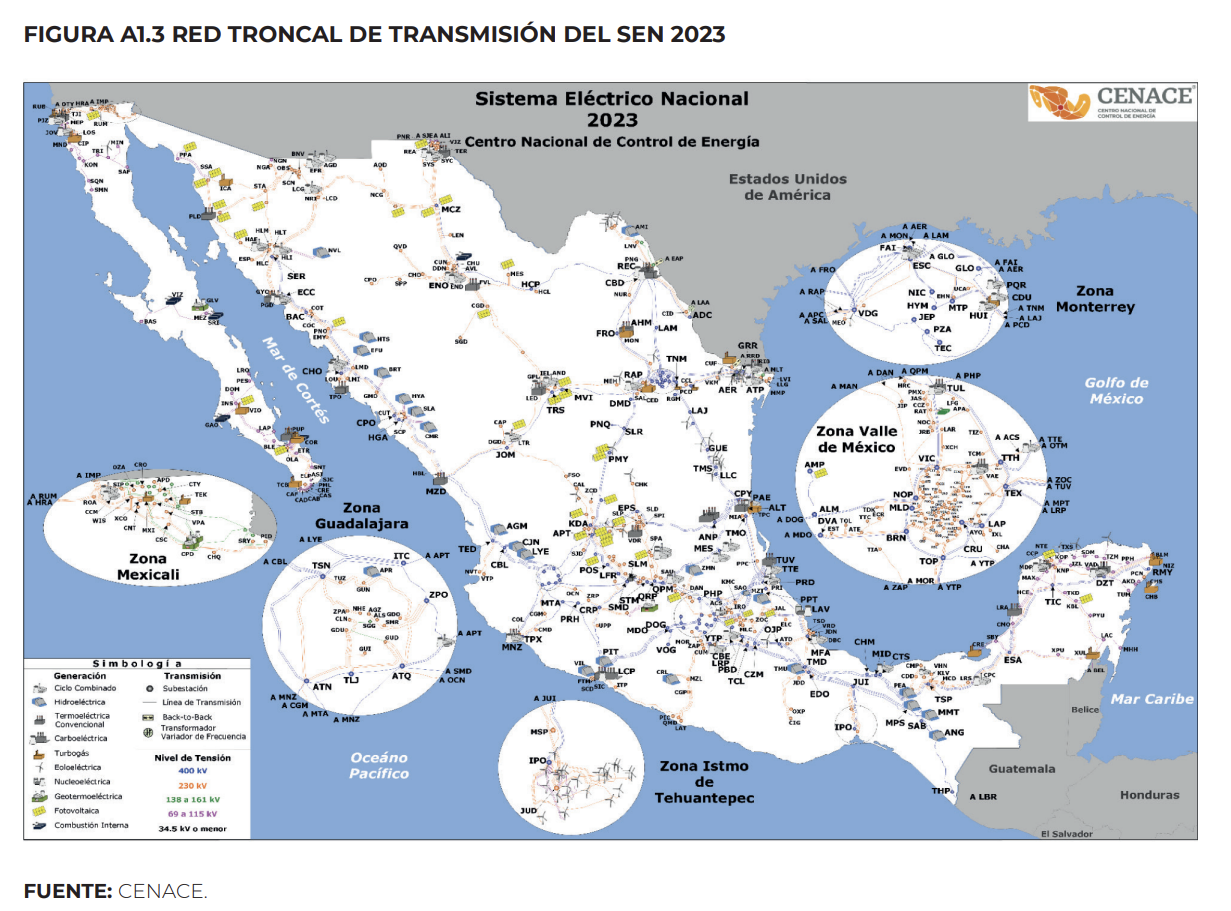
\includegraphics[width=\textwidth,height=0.72\textheight,keepaspectratio]{figuras/04_metodologia/red_troncal_sen_2023.png}
\caption{Red troncal de transmisión del SEN en 2023. Imagen incorporada en \texttt{micode.ipynb}, figura AI.3. La fuente indicada en la imagen es CENACE.}
\label{fig:red-troncal-sen}
\end{figure}

La figura~\ref{fig:red-troncal-sen} presenta la distribución de infraestructura de generación y transmisión, con símbolos para diferentes tecnologías y niveles de tensión. Sus ampliaciones permiten observar zonas como Mexicali, Guadalajara, Monterrey, Valle de México e Istmo de Tehuantepec. Este contexto ayuda a interpretar las columnas de sistema y área como identificadores territoriales del registro eléctrico.

\begin{figure}[p]
\centering
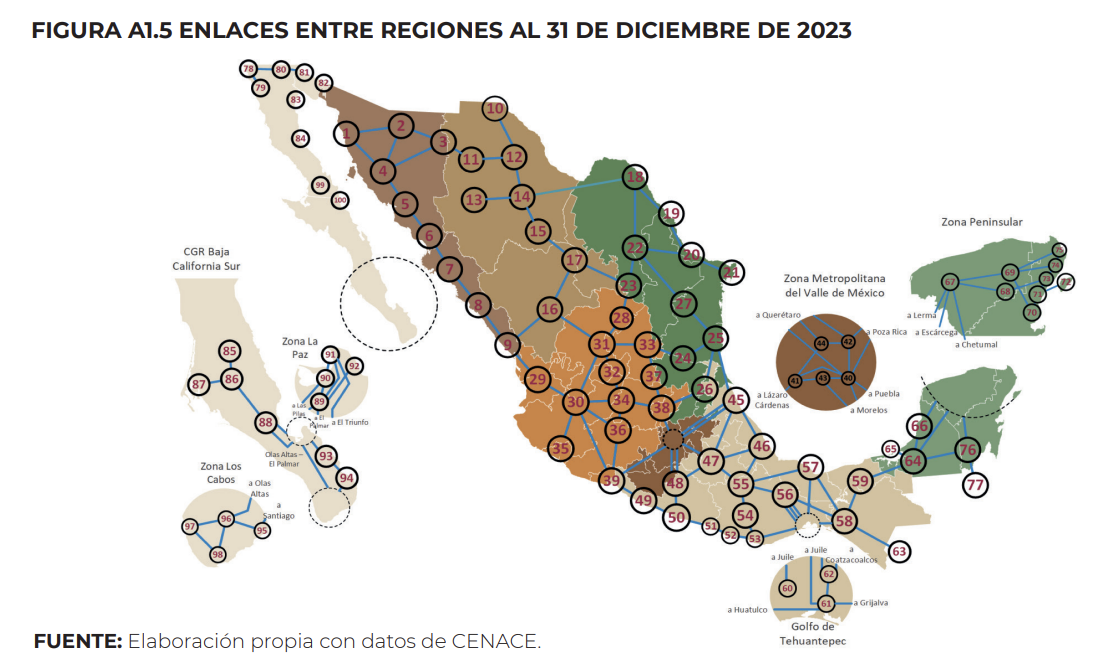
\includegraphics[width=\textwidth,height=0.68\textheight,keepaspectratio]{figuras/04_metodologia/enlaces_regiones_2023.png}
\caption{Enlaces entre regiones al 31 de diciembre de 2023. Imagen incorporada en \texttt{micode.ipynb}, figura AI.5. El crédito original señala una elaboración con datos de CENACE; el mapa se reproduce del cuaderno y no constituye una elaboración de esta tesis.}
\label{fig:enlaces-regiones}
\end{figure}

La figura~\ref{fig:enlaces-regiones} representa regiones numeradas y los enlaces dibujados entre ellas, e incluye detalles de Baja California Sur y de la Zona Metropolitana del Valle de México. Los números del mapa no deben interpretarse como equivalentes directos a los nueve códigos de área del archivo, pues esa correspondencia requiere información adicional.

En las salidas del cuaderno se identifican los sistemas BCA, BCS y SIN, así como las áreas BCA, BCS, CEN, NES, NOR, NTE, OCC, ORI y PEN. Los mapas complementan la descripción de estos registros. El modelo OLS utiliza la generación de una sola área y no incorpora coordenadas, distancias ni enlaces de transmisión como variables predictoras.

